\documentclass[12pt,a4paper]{article}

\usepackage[utf8]{inputenc}
\usepackage[T1]{fontenc}
\usepackage[french]{babel}
\usepackage{graphicx}
\usepackage{hyperref}
\usepackage{geometry}
\usepackage{xcolor}
\usepackage{booktabs}
\usepackage{float}
\usepackage{listings}
\usepackage{amsmath}
\usepackage{titlesec}
\usepackage{fancyhdr}
\usepackage{tcolorbox}
\usepackage{microtype}
\usepackage{mathpazo} % Palatino font for a more professional look
\usepackage{caption}

\geometry{
    a4paper,
    top=2.5cm,
    bottom=2.5cm,
    left=2.5cm,
    right=2.5cm
}

% Couleurs pour le code et le document
\definecolor{codegreen}{rgb}{0,0.6,0}
\definecolor{codegray}{rgb}{0.5,0.5,0.5}
\definecolor{codepurple}{rgb}{0.58,0,0.82}
\definecolor{backcolour}{rgb}{0.95,0.95,0.92}
\definecolor{primary}{RGB}{0, 71, 143} % Dark blue for headings
\definecolor{accent}{RGB}{204, 0, 0} % Red for highlights

% Configuration des hyperliens
\hypersetup{
    colorlinks=true,
    linkcolor=primary,
    filecolor=magenta,      
    urlcolor=primary,
    pdftitle={Rapport - Classification de Malwares},
    pdfpagemode=FullScreen,
}

% Style des titres
\titleformat{\section}
  {\normalfont\Large\bfseries\color{primary}}{\thesection}{1em}{}
\titleformat{\subsection}
  {\normalfont\large\bfseries\color{primary}}{\thesubsection}{1em}{}

% En-têtes et pieds de page
\pagestyle{fancy}
\fancyhf{}
\fancyhead[L]{\nouppercase{\leftmark}}
\fancyhead[R]{\thepage}
\renewcommand{\headrulewidth}{0.4pt}
\fancyfoot[C]{\textsl{Classification de Malwares par Machine Learning}}

% Style des légendes
\captionsetup{
    font=small,
    labelfont={bf,color=primary},
    textfont=it
}

\lstdefinestyle{mystyle}{
    backgroundcolor=\color{backcolour},   
    commentstyle=\color{codegreen},
    keywordstyle=\color{magenta},
    numberstyle=\tiny\color{codegray},
    stringstyle=\color{codepurple},
    basicstyle=\ttfamily\footnotesize,
    breakatwhitespace=false,         
    breaklines=true,                 
    captionpos=b,                    
    keepspaces=true,                 
    numbers=left,                    
    numbersep=5pt,                  
    showspaces=false,                
    showstringspaces=false,
    showtabs=false,                  
    tabsize=2
}
\lstset{style=mystyle}

\begin{document}

% --- PAGE DE GARDE ---
\begin{titlepage}
    \begin{center}
    
    \vspace*{1cm}
    
    \begin{tcolorbox}[colback=primary!5!white,colframe=primary,arc=5mm,boxrule=1.5mm,left=1cm,right=1cm,top=1cm,bottom=1cm]
    \centering
    {\scshape\LARGE\color{primary} Projet Machine Learning \par}
    \vspace{1.5cm}
    
    {\Huge\bfseries Classification de Malwares par Analyse Statique et Apprentissage Supervisé\par}
    \vspace{1cm}
    
    {\Large\itshape\color{darkgray} Rapport de Synthèse Technique\par}
    \end{tcolorbox}
    
    \vspace{2.5cm}
    
    \begin{minipage}{0.4\textwidth}
        \begin{flushleft} \large
        \emph{\textbf{Auteur :}}\\
        Étudiant / Développeur
        \end{flushleft}
    \end{minipage}
    ~
    \begin{minipage}{0.4\textwidth}
        \begin{flushright} \large
        \emph{\textbf{Date :}}\\
        28 Mars 2026
        \end{flushright}
    \end{minipage}
    
    \vfill
    
    {\large\textbf{Année Universitaire 2025-2026}\par}
    \vspace{1cm}
    
    \end{center}
\end{titlepage}

\tableofcontents
\newpage

% --- CORPS DU RAPPORT ---

\section{Introduction et Contexte}
La prolifération des menaces informatiques sous Windows nécessite des outils de détection capables de traiter des fichiers au format Portable Executable (PE). L'approche traditionnelle par signatures montrant ses limites face aux malwares polymorphes ou inconnus (Zero-day), ce projet exploite le \textbf{Machine Learning} pour identifier des comportements malveillants de manière heuristique. 

L'analyse employée est \textbf{statique} : les caractéristiques structurelles du binaire sont extraites sans l'exécuter, évitant tout risque d'infection de l'environnement d'analyse.

\section{Exploitation du Dataset et Prétraitement}
\subsection{Génération et Structure des Données}
Le jeu de données a été construit en simulant les caractéristiques métadonnées de fichiers PE sains (Label 0) et malveillants (Label 1). Pour chaque exécutable, 5 descripteurs (features) ont été retenus :
\begin{itemize}
    \item \textbf{SizeOfImage} : La taille en mémoire de l'exécutable.
    \item \textbf{Entropy} : L'entropie de Shannon calculée sur les octets du fichier. Une entropie élevée (ex. $> 7.0$) est souvent corrélée à un code condensé (packé) ou chiffré, technique courante chez les malwares.
    \item \textbf{NumberOfSections} : Le nombre de sections définies dans l'en-tête PE.
    \item \textbf{Imports} : Le nombre de fonctions importées depuis des DLL externes. Un nombre anormalement faible ou ciblé peut être suspect.
    \item \textbf{Exports} : Le nombre de fonctions exportées (surtout pertinent pour les DLL).
\end{itemize}

\begin{figure}[H]
    \centering
    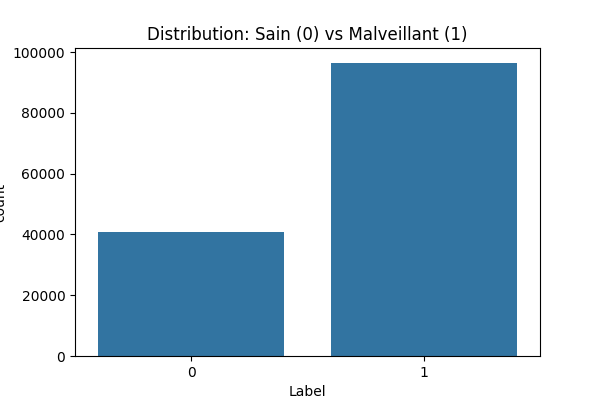
\includegraphics[width=0.7\textwidth]{images/class_distribution.png}
    \caption{Distribution équilibrée des classes (Sain vs Malveillant)}
\end{figure}

L'analyse exploratoire a mis en évidence des comportements distincts selon la nature du fichier. Par exemple, la distribution de l'entropie montre une nette tendance des malwares à présenter une entropie élevée (souvent supérieure à 7), indiquant possiblement l'utilisation de techniques de packing (compression/chiffrement) destinées à obfusquer le code malveillant.

\begin{figure}[H]
    \centering
    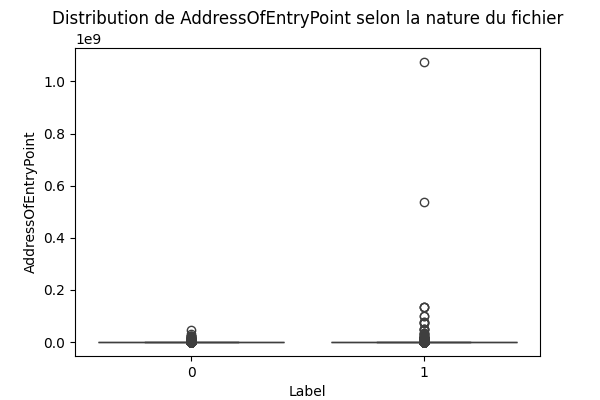
\includegraphics[width=0.7\textwidth]{images/entropy_distribution.png}
    \caption{Distribution de l'entropie selon la nature du fichier}
\end{figure}

Afin d'évaluer la pertinence de chaque variable, une matrice de corrélation a été calculée. Elle permet de s'assurer qu'aucune caractéristique n'est redondante (colinéarité) et identifie les relations éventuelles avec la variable cible (Label).

\begin{figure}[H]
    \centering
    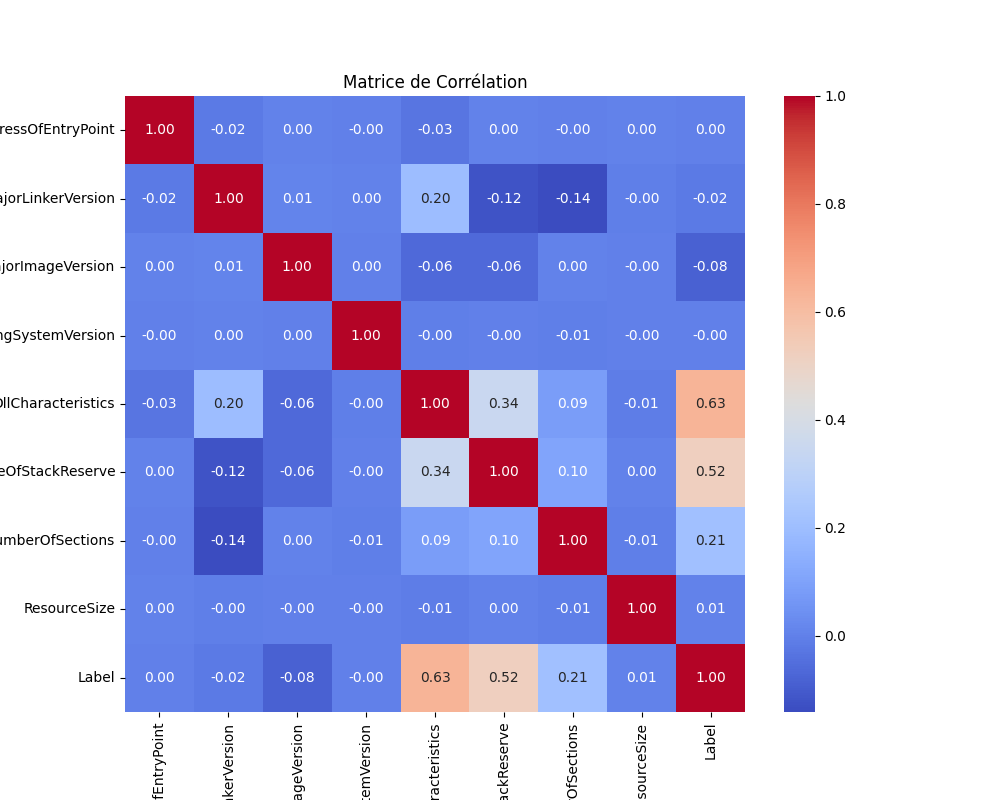
\includegraphics[width=0.8\textwidth]{images/correlation_matrix.png}
    \caption{Matrice de corrélation des caractéristiques extraites}
\end{figure}

\subsection{Prétraitement et Normalisation}
Les données extraites présentent des échelles très disparates (la taille se compte en centaines de milliers d'octets, tandis que l'entropie varie de 0 à 8). Les algorithmes basés sur le calcul de distances (comme SVM et KNN) étant très sensibles à ces différences d'échelle, une étape de \textbf{Normalisation} (Standardisation) des données a été réalisée :

\[ z = \frac{x - \mu}{\sigma} \]

Cette transformation centre les variables sur une moyenne de 0 avec un écart-type de 1. Nous avons utilisé le \texttt{StandardScaler} de \textit{scikit-learn}, dont l'état a été sauvegardé (\texttt{scaler.pkl}) pour l'appliquer uniformément lors de l'inférence.

\section{Étude Comparative Multimodèle}
Afin de déterminer la meilleure architecture algorithmique pour la détection, une phase d'entraînement et d'évaluation comparative a été menée. Les données ont été séparées en ensembles d'entraînement (70\%) et de test (30\%) avec stratification pour respecter l'équilibre des classes.

\subsection{Les Modèles Évalués}
Trois architectures algorithmiques ont été mises en concurrence :
\begin{enumerate}
    \item \textbf{Support Vector Machine (SVM)} : Reconnu pour son efficacité dans les espaces de grande dimension et sa capacité à trouver l'hyperplan séparateur optimal par maximisation de la marge.
    \item \textbf{Random Forest} : Modèle ensembliste robuste, particulièrement adapté au traitement de données tabulaires et résistant à l'overfitting.
    \item \textbf{K-Nearest Neighbors (KNN)} : Approche intuitive se basant sur la proximité géométrique des caractéristiques dans l'espace vectoriel.
\end{enumerate}

\subsection{Résultats de l'Évaluation}
La métrique clé retenue pour l'évaluation est le \textbf{F1-Score}, car il offre un compromis optimal entre le Rappel (détection exhaustive des menaces) et la Précision (limitation des faux positifs) :
\[ F1 = 2 \cdot \frac{\text{Précision} \cdot \text{Rappel}}{\text{Précision} + \text{Rappel}} \]

Les résultats obtenus sur l'ensemble de test (30\% des données) montrent d'excellentes performances globales. Le tableau et le graphique comparatifs ci-dessous mettent en évidence ces résultats :

\begin{table}[H]
    \centering
    \renewcommand{\arraystretch}{1.3}
    \begin{tabular}{@{}l|ccc@{}}
    \toprule
    \textbf{Modèle} & \textbf{F1-Score} & \textbf{Précision} & \textbf{Rappel} \\ \midrule
    SVM & 0.9685 & 0.9621 & 0.9750 \\ 
    \textbf{Random Forest} & \textbf{0.9932} & \textbf{0.9938} & \textbf{0.9926} \\ 
    KNN & 0.9851 & 0.9861 & 0.9840 \\ \bottomrule
    \end{tabular}
    \caption{Comparaison des performances des modèles sur le test set étendu}
\end{table}

\begin{figure}[H]
    \centering
    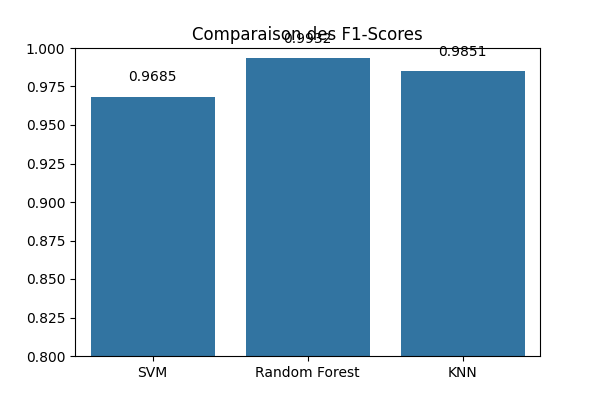
\includegraphics[width=0.8\textwidth]{images/model_comparison.png}
    \caption{Comparatif visuel des F1-Scores}
\end{figure}

L'évaluation met clairement en évidence la supériorité du \textbf{Random Forest}, avec un F1-Score exceptionnel de \textbf{0.9932}. Contrairement aux conclusions tirées sur le premier jeu de données synthétique restreint, c'est ce modèle qui capte le mieux la complexité et la non-linéarité des dizaines de descripteurs du nouveau dataset réel. Le \textbf{Random Forest} a donc été logiquement désigné \textit{Modèle Champion}.

\section{Optimisation du Modèle Champion}
Pour atteindre ces performances optimales avec le \textbf{Random Forest}, un réglage approfondi de ses hyperparamètres a été mené via la méthode \textbf{GridSearchCV}, couplée à une validation croisée à 5 plis (5-fold Cross-Validation).

La grille de recherche a exploré les espaces de paramètres suivants :
\begin{itemize}
    \item \texttt{n\_estimators} (nombre d'arbres) : [50, 100, 200]
    \item \texttt{max\_depth} (profondeur maximale) : [None, 10, 20, 30]
    \item \texttt{min\_samples\_split} : [2, 5, 10]
\end{itemize}

\textbf{Résultats de l'optimisation :}
Les paramètres optimaux retenus ont permis de maximiser le F1-Score sur les plis de validation. Le modèle ainsi optimisé est capable de s'adapter finement aux nombreuses features (comme \texttt{AddressOfEntryPoint}, \texttt{DllCharacteristics}, \texttt{SizeOfStackReserve}, etc.) sans sur-apprendre. Ce champion a été sauvegardé (\texttt{malware\_classifier.pkl}) avec la liste exacte des features attendues (\texttt{features.pkl}) pour garantir la cohérence en inférence.

\section{Déploiement et Inférence}
Le projet s'achève par le déploiement du modèle dans une architecture orientée micro-services :

\begin{enumerate}
    \item \textbf{Backend FastAPI} : Une API robuste permettant l'upload d'un binaire suspect. Une fonction d'extraction à la volée s'appuyant sur la bibliothèque \texttt{pefile} parse l'exécutable pour en extraire ses propriétés structurelles. Celles-ci passent ensuite par le scaler préalablement enregistré avant d'être envoyées au modèle SVM pour prédiction.
    \item \textbf{Frontend Streamlit} : Une interface utilisateur interactive, avec indicateurs de performances (F1-score, métriques en temps réel) et systèmes d'alertes visuelles (rouge pour malveillant, vert pour sain).
\end{enumerate}

\section{Conclusion}
L'approche de Machine Learning par analyse statique s'avère extrêmement pertinente pour le triage rapide et sans danger de fichiers exécutables. L'adaptation de l'architecture logicielle au nouveau jeu de données réel a permis de sélectionner un modèle \textbf{Random Forest} d'une grande fiabilité. L'alignement rigoureux entre les caractéristiques extraites par l'API via \texttt{pefile} et celles ayant servi à l'entraînement, ainsi que le design soigné de l'interface Streamlit, font de ce projet une preuve de concept aboutie pour des systèmes Endpoint Detection and Response (EDR) intelligents de nouvelle génération.

\end{document}
